\documentclass{article}
\usepackage[utf8]{inputenc}
\usepackage[greek,english]{babel}
\usepackage{alphabeta}
\usepackage{fancyhdr}
\usepackage{listings}
\usepackage{mathtools}
\usepackage{siunitx}
\usepackage{xcolor}
\usepackage{graphicx}
\usepackage{pgfplots}
\usepackage[export]{adjustbox}
\usepackage{biblatex}
\addbibresource{dl2-citations.bib}

%\pagestyle{fancy}
%\renewcommand\headrulewidth{0pt}
%\fancyhead{}
%\fancyfoot{}
%\fancyfoot[R]{\thepage}

\title{Εργαστηριακή Εργασία 2 - Αθροιστές-Αφαιρέτες}
\author{Χρήστος Μαργιώλης - 19390133 \\ Τμήμα 8}
\date{Ιούνιος 2020}

\begin{document}

\begin{figure}[t!]
    \centering
    
\includegraphics[scale=0.3, center]{./res/Logo_University_of_West_Attica.png}
    \Large
    \textbf{Πανεπιστήμιο Δυτικής Αττικής} \\
    \large
    Τμήμα Μηχανικών Πληροφορικής και Ηλεκτρονικών Υπολογιστών \\
    Ψηφιακή Σχεδίαση
\end{figure}
\begin{figure}[b]
    \centering
    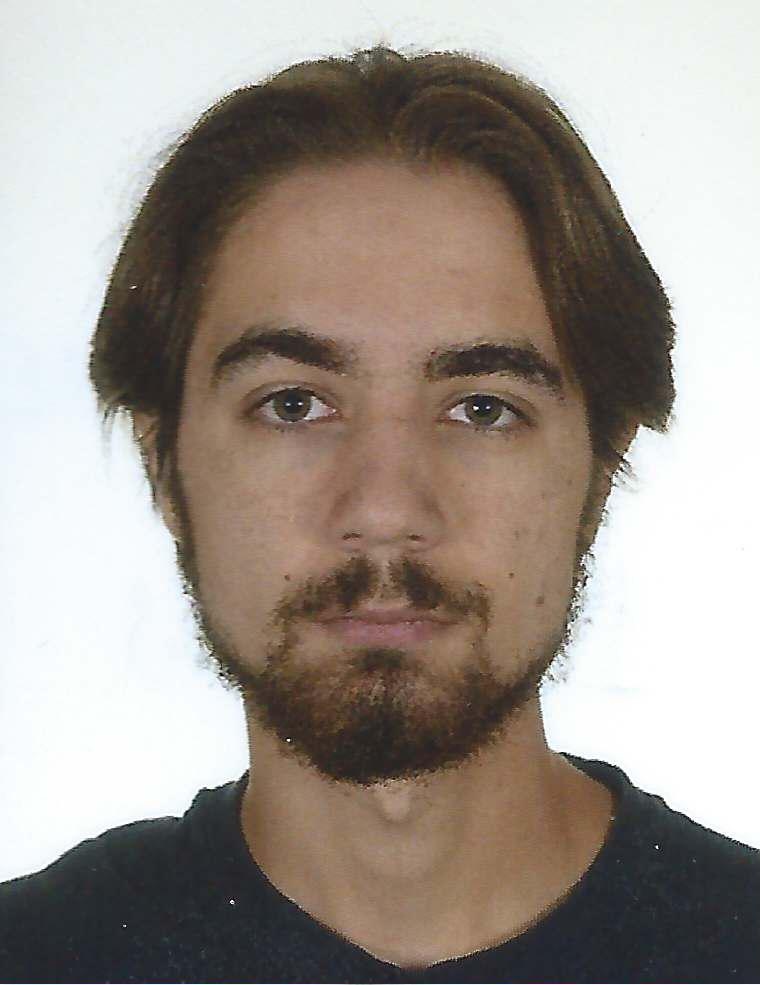
\includegraphics[scale=1]{./res/19390133.jpeg}
\end{figure}

\begin{titlepage}
\maketitle
\end{titlepage}

\renewcommand{\contentsname}{Περιεχόμενα}
\tableofcontents

\renewcommand{\abstractname}{Εισαγωγή}
\begin{abstract}
	Το αντικείμενο της εργασίας αυτής είναι η κατανόηση και η εφαρμογή
	των λογικών κυκλωμάτων υπεύθυνων για προσθέσεις και αφαιρέσεις - τους
	αθροιστές και τους αφαιρέτες.
\end{abstract}
\pagebreak

\section{Συλλογή βιβλιογραφίας}
Η βιβλιογραφία που χρησιμοποιήθηκε κάλυψε τα βασικά προβλήματα της εργασίας,
δηλαδή τις έννοιες και τις λειτουργίες των αθροιστών και αφαιρετών.

\section{Περιγραφή υλοποίησης}
Για την υλοποίηση της εργασίας και βασισμένος στην βιβλιογραφία που συνέλεξα,
χρησιμοποιήσα κυκλώματα προσθετών και αφαιρετών, καθώς και ολοκληρωμένα κυκλώματα και
block διαγράμματα.
Επίσης χρησιμοποιήθηκαν πίνακες αλήθειας και λογικές εξισώσεις για τις επαληθεύσεις
των αποτελεσμάτων και των μετρήσεων.

\section{Θεωρητικό μέρος}
Άθροιστες και αφαιρέτες είναι λογικά κυκλώματα που έχουν την ιδιότητα να προσθέτουν
και να αφαιρούν bits αντίστοιχα, όπως λέει και το όνομα τους. Στην απλούστερη μορφή του,
ένα κύκλωμα πρόσθεσης/αφαίρεσης ονομάζεται ημιαθροιστής/ημιαφαιρέτης. Προκειμένου να
μπορέσουμε να κάνουμε πλήρης προσθέσεις και αφαιρέσεις χρησιμοποιούμε πιο εκτεταμένες
μορφές των παραπάνω κυκλωμάτων τις οποίες ονομάζουμε πλήρεις αθροιστές/αφαιρέτες.

\section{Εργαστηριακό μέρος}

Λόγω του ότι οι εικόνες καταλαμβάνουν πολύ χώρο, στις 4 πρώτες ασκήσεις για κάθε
κύκλωμα θα βάλω μία εικόνα και θα αναλύσω όλες τις υπόλοιπες καταστάσεις και εξόδους
μέσα από τις λογικές τους εξισώσεις. Όπου η εξίσωση δίνει αποτέλεσμα 1 σημαίνει ότι
στο κύκλωμα θα ανάψει το LED που είναι συνδεδεμένο στην έξοδο που έδωσε λογικό 1, και
όπου δίνει αποτέλεσμα 0 σημαίνει οτι δεν θα ανάψει το LED στην έξοδο του κυκλώματος
αντίστοιχα.

\subsection{Ημιαθροιστής}

Ο πίνακας αλήθειας για τον ημιαθροιστή είναι ο παρακάτω

\begin{center}
	\begin{tabular}{|c|c|c|c|}
	\hline
	$X$ & $Y$ & $S$ & $C$ \\
	\hline
	0 & 0 & 0 & 0 \\
	0 & 1 & 1 & 0 \\
	1 & 0 & 1 & 0 \\
	1 & 1 & 0 & 1 \\
	\hline
\end{tabular}
\end{center}

Οι λογικές εξισώσεις για το άθροισμα και το κρατούμενο που προκύπτουν από τον πίνακα
αληθείας είναι οι εξής

\[S = \overline{X} \cdot Y + X \cdot \overline{Y} = X \oplus Y\]
\[C = X \cdot Y\]

Θα αναλύσουμε τις εξόδους για κάθε πιθανό συνδυασμό εισόδων στο παρακάτω κύκλωμα. \\

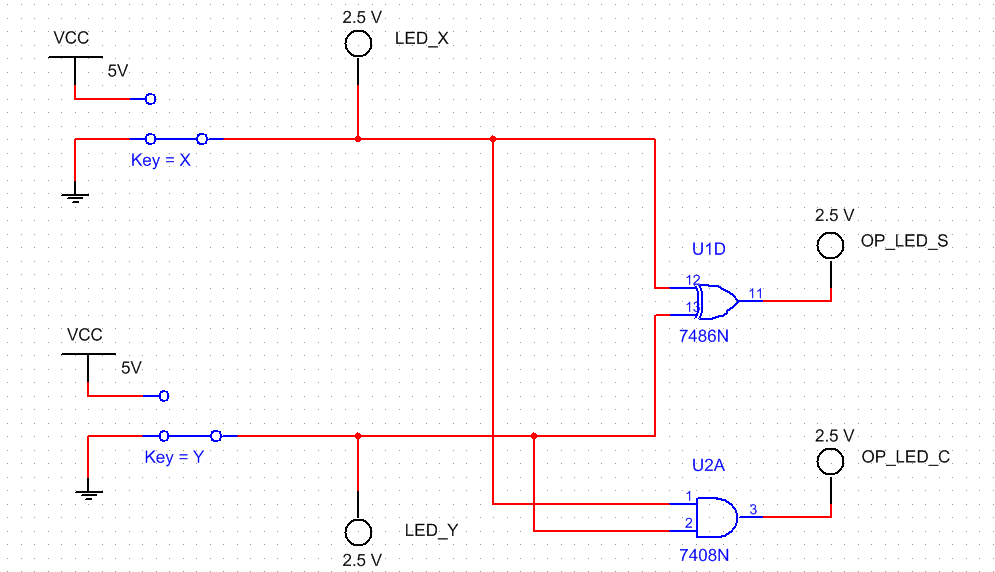
\includegraphics[width=\textwidth]{./res/ha00.png}

\begin{itemize}
	\item
	$X = 0$ \\
	$Y = 0$

	\[S = 0 \oplus 0 = 0\]
	\[C = 0 \cdot 0 = 0\]

	\item
	$X = 0$ \\
	$Y = 1$

	\[S = 0 \oplus 1 = 1\]
	\[C = 0 \cdot 1 = 0\]

	\item
	$X = 1$ \\
	$Y = 0$

	\[S = 1 \oplus 0 = 1\]
	\[C = 1 \cdot 0 = 0\]

	\item
	$X = 1$ \\
	$Y = 1$

	\[S = 1 \oplus 1 = 0\]
	\[C = 1 \cdot 1 = 1\]
\end{itemize}

\subsection{Ημιαφαιρέτης}

Ο πίνακας αλήθειας για τον ημιαφαιρέτη είναι ο παρακάτω

\begin{center}
	\begin{tabular}{|c|c|c|c|}
	\hline
	$X$ & $Y$ & $D$ & $B$ \\
	\hline
	0 & 0 & 0 & 0 \\
	0 & 1 & 1 & 1 \\
	1 & 0 & 1 & 0 \\
	1 & 1 & 0 & 0 \\
	\hline
\end{tabular}
\end{center}

Οι λογικές εξισώσεις για την διαφορά και το δανειζόμενο που προκύπτουν από τον πίνακα
αληθείας είναι οι εξής

\[S = \overline{X} \cdot Y + X \cdot \overline{Y} = X \oplus Y\]
\[C = \overline{X} \cdot Y\]

Θα αναλύσουμε τις εξόδους για κάθε πιθανό συνδυασμό εισόδων στο παρακάτω κύκλωμα. \\

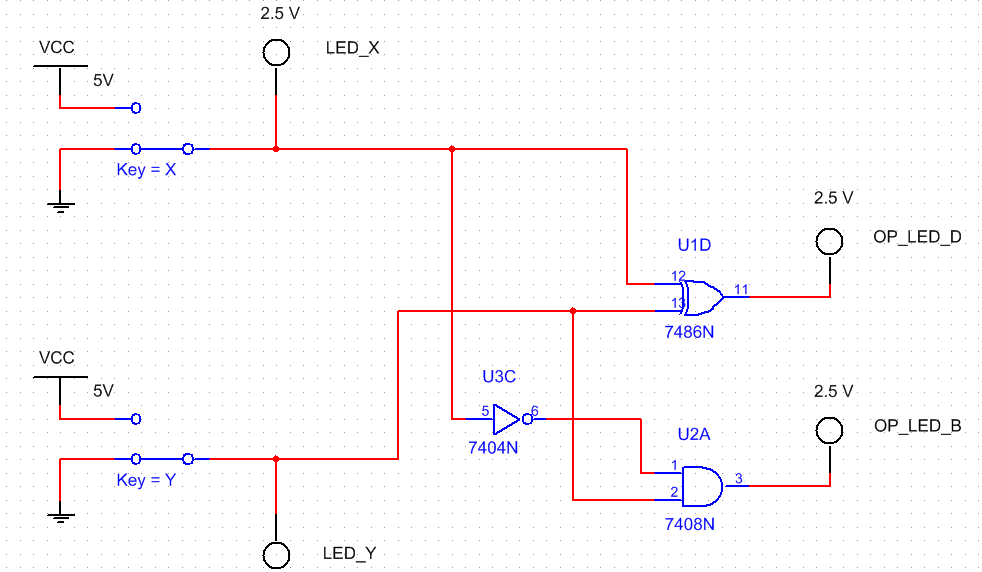
\includegraphics[width=\textwidth]{./res/hs00.png}

\begin{itemize}
	\item
	$X = 0$ \\
	$Y = 0$

	\[S = 0 \oplus 0 = 0\]
	\[C = \overline{0} \cdot 0 = 1 \cdot 0 = 0\]

	\item
	$X = 0$ \\
	$Y = 1$

	\[S = 0 \oplus 1 = 1\]
	\[C = \overline{0} \cdot 1 = 1 \cdot 1 = 1\]

	\item
	$X = 1$ \\
	$Y = 0$

	\[S = 1 \oplus 0 = 1\]
	\[C = \overline{1} \cdot 0 = 0 \cdot 0 = 0\]

	\item
	$X = 1$ \\
	$Y = 1$

	\[S = 1 \oplus 1 = 0\]
	\[C = \overline{1} \cdot 1 = 0 \cdot 1 = 0\]
\end{itemize}

\subsection{Πλήρης Αθροιστής}

Ο πίνακας αλήθειας για τον πλήρη αθροιστή είναι ο παρακάτω

\begin{center}
	\begin{tabular}{|c|c|c|c|c|c|}
	\hline
	$X_n$ & $Y_n$ & $C_{n-1}$ & $S_n$ & $C_n$ \\
	\hline
	0 & 0 & 0 & 0 & 0 \\
	0 & 0 & 1 & 1 & 0 \\
	0 & 1 & 0 & 1 & 0 \\
	0 & 1 & 1 & 0 & 1 \\
	1 & 0 & 0 & 1 & 0 \\
	1 & 0 & 1 & 0 & 1 \\
	1 & 1 & 0 & 0 & 1 \\
	1 & 1 & 1 & 1 & 1 \\
	\hline
\end{tabular}
\end{center}

Οι λογικές εξισώσεις στην τελική τους μορφή για το άθροισμα και το κρατούμενο που
προκύπτουν από τον πίνακα αληθείας είναι οι εξής

\[S_n = X_n \oplus Y_n \oplus C_{n-1}\]
\[C_n = (X_n \oplus Y_n)C_{n-1} + X_n \cdot Y_n\]

Θα αναλύσουμε τις εξόδους για κάθε πιθανό συνδυασμό εισόδων στο παρακάτω κύκλωμα. \\
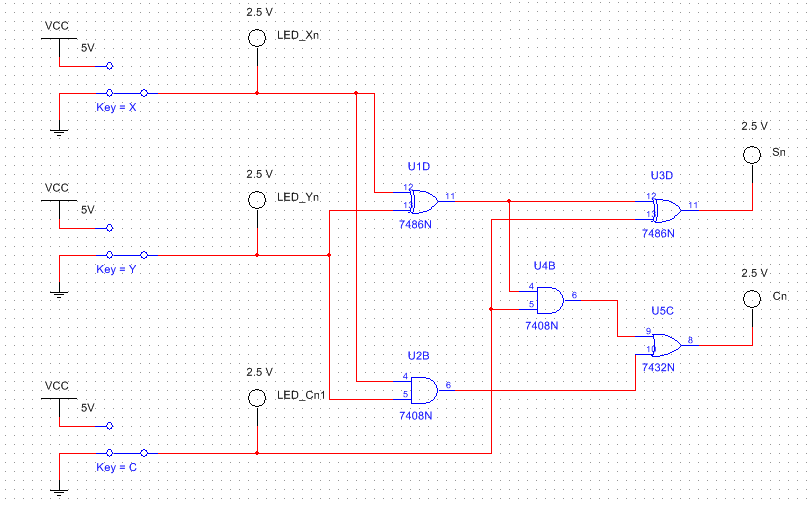
\includegraphics[width=\textwidth]{./res/fa000.png}

\begin{itemize}
	\item
	$X_n = 0$ \\
	$Y_n = 0$ \\
	$C_{n-1} = 0$

	\[S_n = 0 \oplus 0 \oplus 0 = 0\]
	\[C_n = (0 \oplus 0)0 + 0 \cdot 0 = 0 \cdot 0 + 0 \cdot 0 = 0\]

	\item
	$X_n = 0$ \\
	$Y_n = 0$ \\
	$C_{n-1} = 1$

	\[S_n = 0 \oplus 0 \oplus 1 = (0 \oplus 0) \oplus 1 = 0 \oplus 1 = 1\]
	\[C_n = (0 \oplus 0)1 + 0 \cdot 0 = 0 \cdot 1 = 0\]

	\item
	$X_n = 0$ \\
	$Y_n = 1$ \\
	$C_{n-1} = 0$

	\[S_n = 0 \oplus 1 \oplus 0 = (0 \oplus 1) \oplus 0 = 1 \oplus 0 = 1\]
	\[C_n = (0 \oplus 1)0 + 0 \cdot 1 = 1 \cdot 0 = 0\]

	\item
	$X_n = 0$ \\
	$Y_n = 1$ \\
	$C_{n-1} = 1$

	\[S_n = 0 \oplus 1 \oplus 1 = (0 \oplus 1) \oplus 1 = 1 \oplus 1 = 0\]
	\[C_n = (0 \oplus 1)1 + 0 \cdot 1 = 1 \cdot 1 = 1\]

	\item
	$X_n = 1$ \\
	$Y_n = 0$ \\
	$C_{n-1} = 0$

	\[S_n = 1 \oplus 0 \oplus 0 = (1 \oplus 0) \oplus 0 = 1 \oplus 0 = 1\]
	\[C_n = (1 \oplus 0)0 + 1 \cdot 0 = 1 \cdot 0 = 0\]

	\item
	$X_n = 1$ \\
	$Y_n = 0$ \\
	$C_{n-1} = 1$

	\[S_n = 1 \oplus 0 \oplus 1 = (1 \oplus 0) \oplus 1 = 1 \oplus 1 = 0\]
	\[C_n = (1 \oplus 0)1 + 1 \cdot 0 = 1 \cdot 1 = 1\]

	\item
	$X_n = 1$ \\
	$Y_n = 1$ \\
	$C_{n-1} = 0$

	\[S_n = 1 \oplus 1 \oplus 0 = (1 \oplus 1) \oplus 0 = 0 \oplus 0 = 0\]
	\[C_n = (1 \oplus 1)0 + 1 \cdot 1 = 1\]

	\item
	$X_n = 1$ \\
	$Y_n = 1$ \\
	$C_{n-1} = 1$

	\[S_n = 1 \oplus 1 \oplus 1 = (1 \oplus 1) \oplus 1 = 0 \oplus 1 = 1\]
	\[C_n = (1 \oplus 1)1 + 1 \cdot 1 = 1 + 1 = 1\]
\end{itemize}

\subsection{Πλήρης Αφαιρέτης}

Ο πίνακας αλήθειας για τον πλήρη αφαιρέτη είναι ο παρακάτω

\begin{center}
	\begin{tabular}{|c|c|c|c|c|c|}
	\hline
	$X_n$ & $Y_n$ & $B_{n-1}$ & $D_n$ & $B_n$ \\
	\hline
	0 & 0 & 0 & 0 & 0 \\
	0 & 0 & 1 & 1 & 1 \\
	0 & 1 & 0 & 1 & 1 \\
	0 & 1 & 1 & 0 & 1 \\
	1 & 0 & 0 & 1 & 0 \\
	1 & 0 & 1 & 0 & 0 \\
	1 & 1 & 0 & 0 & 0 \\
	1 & 1 & 1 & 1 & 1 \\
	\hline
\end{tabular}
\end{center}

Οι λογικές εξισώσεις στην τελική τους μορφή για το άθροισμα και το κρατούμενο που
προκύπτουν από τον πίνακα αληθείας είναι οι εξής

\[D_n = X_n \oplus Y_n \oplus B_{n-1}\]
\[B_n = \overline{(X_n \oplus Y_n)}B_{n-1} + \overline{X_n} \cdot Y_n\]

Θα αναλύσουμε τις εξόδους για κάθε πιθανό συνδυασμό εισόδων στο παρακάτω κύκλωμα. \\
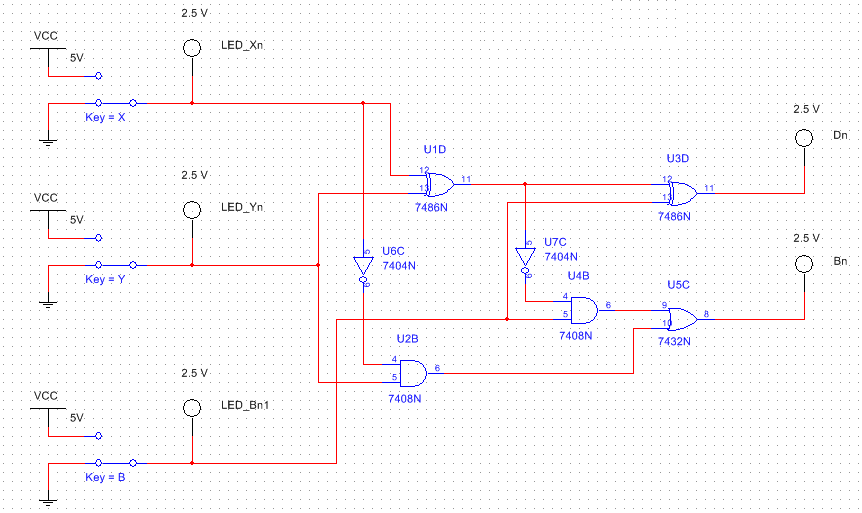
\includegraphics[width=\textwidth]{./res/fs000.png}

\begin{itemize}
	\item
	$X_n = 0$ \\
	$Y_n = 0$ \\
	$B_{n-1} = 0$

	\[D_n = 0 \oplus 0 \oplus 0 = 0\]
	\[B_n = \overline{(0 \oplus 0)}0 + \overline{0} \cdot 0 =
		1 \cdot 0 + 1 \cdot 0 = 0\]

	\item
	$X_n = 0$ \\
	$Y_n = 0$ \\
	$B_{n-1} = 1$

	\[D_n = 0 \oplus 0 \oplus 1 = (0 \oplus 0) \oplus 1 = 0 \oplus 1 = 1\]
	\[B_n = \overline{(0 \oplus 0)}1 + \overline{0} \cdot 0 =
		1 \cdot 1 + 1 \cdot 0 = 1\]

	\item
	$X_n = 0$ \\
	$Y_n = 1$ \\
	$B_{n-1} = 0$

	\[D_n = 0 \oplus 1 \oplus 0 = (0 \oplus 1) \oplus 0 = 1 \oplus 0 = 1\]
	\[B_n = \overline{(0 \oplus 1)}0 + \overline{0} \cdot 1 =
		\overline{1} \cdot 0 + 1 \cdot 1 = 1\]

	\item
	$X_n = 0$ \\
	$Y_n = 1$ \\
	$B_{n-1} = 1$

	\[D_n = 0 \oplus 1 \oplus 1 = (0 \oplus 1) \oplus 1 = 1 \oplus 1 = 0\]
	\[B_n = \overline{(0 \oplus 1)}1 + \overline{0} \cdot 1 =
		\overline{1} \cdot 1 + 1 \cdot 1 = 1\]

	\item
	$X_n = 1$ \\
	$Y_n = 0$ \\
	$B_{n-1} = 0$

	\[D_n = 1 \oplus 0 \oplus 0 = (1 \oplus 0) \oplus 0 = 1 \oplus 0 = 1\]
	\[B_n = \overline{(1 \oplus 0)}0 + \overline{1} \cdot 0 =
		\overline{1} \cdot 0 = 0\]

	\item
	$X_n = 1$ \\
	$Y_n = 0$ \\
	$B_{n-1} = 1$

	\[D_n = 1 \oplus 0 \oplus 1 = (1 \oplus 0) \oplus 1 = 1 \oplus 1 = 0\]
	\[B_n = \overline{(1 \oplus 0)}1 + \overline{1} \cdot 0 =
		\overline{1} \cdot 1 = 0\]

	\item
	$X_n = 1$ \\
	$Y_n = 1$ \\
	$B_{n-1} = 0$

	\[D_n = 1 \oplus 1 \oplus 0 = (1 \oplus 1) \oplus 0 = 0 \oplus 0 = 0\]
	\[B_n = \overline{(1 \oplus 1)}0 + \overline{1} \cdot 1 =
		\overline{0} \cdot 0 + 0 \cdot 1 = 0\]

	\item
	$X_n = 1$ \\
	$Y_n = 1$ \\
	$B_{n-1} = 1$

	\[D_n = 1 \oplus 1 \oplus 1 = (1 \oplus 1) \oplus 1 = 0 \oplus 1 = 1\]
	\[B_n = \overline{(1 \oplus 1)}1 + \overline{1} \cdot 1 =
		\overline{0} \cdot 1 + 0 \cdot 1 = 1\]

\end{itemize}

\subsection{Αθροιστής 4-bit}
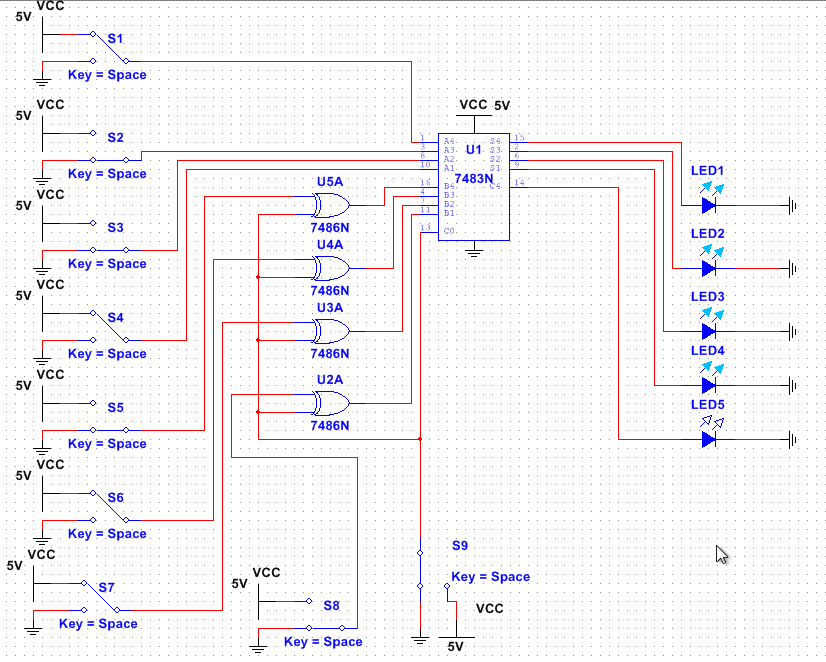
\includegraphics[width=\textwidth]{./res/fa7486.png}

\subsubsection{Είσοδος 0V - Λειτουργία πρόσθεσης}
Από το παραπάνω σχηματικό παρατηρούμε ότι η πράξεις που εκτελεί ο αθροιστής
πράγματι λειτουργούν σωστά - δηλαδή, επαληθεύουν την μαθηματική και θεωρητική
προσέγγιση των πράξεων που εκτελούνται. \\
Στην εικόνα φαίνεται το αποτέλεσμα της πράξης
\[1001 + 0110 = 1111\]
Επειδή δεν υπάρχει κρατούμενο, το πράσινο LED δεν ανάβει. Είναι σημαντικό να 
σημειωθεί ότι το κρατούμενο αυτό προκύπτει επειδή υπάρχει υπερχείλιση (overflow).
Για παράδειγμα στην παρακάτω πράξη $1001 + 1000 = 0001$ το αποτέλεσμα κανονικά 
είναι $10001$ λόγω υπερχείλισης, όμως αγννοούμε το παραπανήσιο bit \cite{efstathiou}. \\
Αντίστοιχα, τα αποτέλεσματα των επόμενων πράξεων που προέκυψαν είναι τα εξής
\begin{itemize}
    \item $1001 + 1000 = 0001$ με κρατούμενο
    \item $1001 + 0100 = 1101$
    \item $1001 + 1100 = 0101$ με κρατούμενο
\end{itemize}

\subsubsection{Είσοδος 5V - Λειτουργία αφαίρεσης}
\begin{itemize}
    \item $1001 - 0111 = 0010$ με κρατούμενο
    \item $1001 - 1111 = 1010$
    \item $1001 - 0100 = 0101$ με κρατούμενο
    \item $1001 - 1011 = 1110$
\end{itemize}

\subsection{Παράλληλος Αθροιστής 4-bit}
\subsubsection{HA για πρόσθεση ψηφίων χαμηλότερης τάξης}
Στην πρόσθεση των ψηφίων χαμηλότερης τάξης χρησιμοποείται Half Adder (ημιαθροιστής)
αντί για Full Adder (πλήρης αθροιστής) επειδή δεν υπάρχει κρατούμενο από προηγούμενη
πράξη.

\subsubsection{Αντικατάσταση HA με FA}
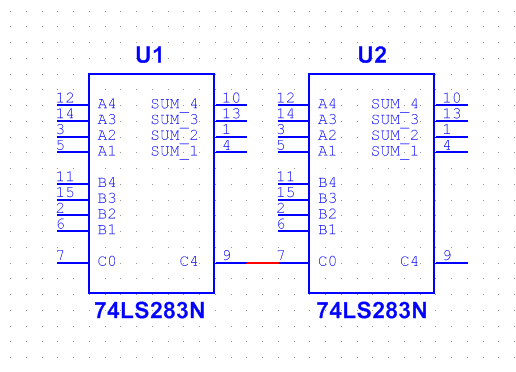
\includegraphics[width=\textwidth]{./res/8bitfa.png}

\subsubsection{Συμπλήρωση τιμών}
Το αποτέλεσμα της πρόσθεσης $1001 + 1011$ είναι $0100$ με κρατούμενο,
οπότε οι τιμές που προκύπτουν είναι οι εξής \\
$S_3 = 0$, $S_2 = 1$, $S_1 = 0$, $S_0 = 0$ και \\
$C_3 = 1$, $C_2 = 0$, $C_1 = 1$, $C_0 = 1$

\subsubsection{Block διάγραμμα πλήρη αθροιστή}
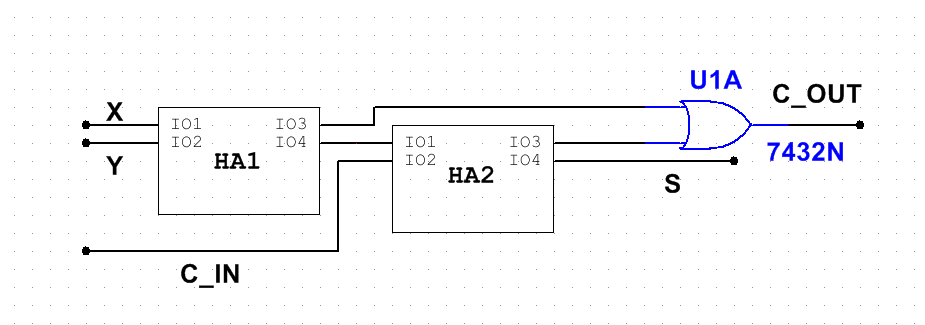
\includegraphics[width=\textwidth]{./res/fablock.png}

\renewcommand\refname{Πηγές}
\printbibliography
\end{document}
